\documentclass[conference]{IEEEtran}

\usepackage{cite}
\usepackage{amsmath,amssymb}
\usepackage{graphicx}
\usepackage{booktabs}
\usepackage{multirow}
\usepackage{array}
\usepackage{url}
\usepackage{xcolor}
\usepackage{balance}
\usepackage{microtype}
\renewcommand{\ttdefault}{cmtt}
\graphicspath{{../figures/}}

% Placeholders: do NOT replace until the corresponding experiment is executed and validated.
\newcommand{\resulttodo}[1]{\textcolor{red}{[INSERT RESULT: #1]}}
\newcommand{\figuretodo}[2]{%
\begin{figure}[!t]
\centering
\fbox{\parbox[c][1.25in][c]{0.92\columnwidth}{\centering #2}}
\caption{#2}
\label{#1}
\end{figure}
}

% Auto-generated numeric macros will be \input from results_macros.tex once experiments finish.
% % Auto-generated by build_macros.py. Do not hand-edit.

\newcommand{\resCompactMLPprecision}{0.743\pm0.037}
\newcommand{\resCompactMLPrecall}{0.904\pm0.016}
\newcommand{\resCompactMLPf}{0.815\pm0.024}
\newcommand{\resCompactMLPfpr}{0.767\pm0.035}
\newcommand{\resCompactMLProcauc}{0.683\pm0.022}
\newcommand{\resLogisticRegressionprecision}{0.719\pm0.043}
\newcommand{\resLogisticRegressionrecall}{0.976\pm0.005}
\newcommand{\resLogisticRegressionf}{0.828\pm0.029}
\newcommand{\resLogisticRegressionfpr}{0.934\pm0.020}
\newcommand{\resLogisticRegressionrocauc}{0.687\pm0.031}
\newcommand{\resRandomForestprecision}{0.760\pm0.035}
\newcommand{\resRandomForestrecall}{0.861\pm0.012}
\newcommand{\resRandomForestf}{0.807\pm0.018}
\newcommand{\resRandomForestfpr}{0.667\pm0.028}
\newcommand{\resRandomForestrocauc}{0.677\pm0.029}
\newcommand{\resXGBoostprecision}{0.762\pm0.036}
\newcommand{\resXGBoostrecall}{0.851\pm0.013}
\newcommand{\resXGBoostf}{0.804\pm0.021}
\newcommand{\resXGBoostfpr}{0.652\pm0.039}
\newcommand{\resXGBoostrocauc}{0.702\pm0.031}
\newcommand{\respayloadonetwoeight}{512}
\newcommand{\respayloadsixteen}{64}
\newcommand{\resLogisticRegressionplatency}{1.11}
\newcommand{\resRandomForestplatency}{51.71}
\newcommand{\resXGBoostplatency}{4.86}
\newcommand{\resCompactMLPplatency}{1.69}
\newcommand{\resRandomForestshapexplainmedian}{881.28}
\newcommand{\resRandomForestshapexplainpersec}{1.13}
\newcommand{\resXGBoostshapexplainmedian}{1.13}
\newcommand{\resXGBoostshapexplainpersec}{888.05}


\title{How Much Telemetry Is Enough? Latency, Payload, and Placement Budgets for Real-Time Intrusion Detection in Digital-Substation Communications}

\author{
\IEEEauthorblockN{Digdarshan Subedi}
\IEEEauthorblockA{
Department of Computer Science\\
University of Wisconsin--Whitewater\\
Whitewater, WI, USA\\
SubediD30@uww.edu}
\and
\IEEEauthorblockN{Nikesh Tiwari}
\IEEEauthorblockA{
School of Business \& Technology\\
Webster University\\
St. Louis, MO, USA\\
nikeshtiwari@webster.edu}
\and
\IEEEauthorblockN{Bibek Ale}
\IEEEauthorblockA{
School of Business \& Technology\\
Webster University\\
St. Louis, MO, USA\\
Bibekale@webster.edu}
}

\begin{document}
\maketitle

\begin{abstract}
Intrusion detection for supervisory control and data acquisition (SCADA) systems is ultimately a real-time communications problem: a detection service is only deployable if the industrial network can deliver enough telemetry, soon enough, for the detector to produce a trustworthy decision within an operational timing envelope. This paper quantifies the three budgets that govern that deployability---end-to-end compute latency, per-record telemetry payload, and feature availability at decision time---for four lightweight machine-learning detectors evaluated on the MSU/ORNL Power System Attack Dataset, with a fifth, a feature-space 1D-CNN from prior work on the same dataset, reported for context but excluded from the new budget experiments (Section~\ref{sec:limitations}). We benchmark batch-size-one preprocessing and inference latency against transfer-time classes derived from IEC~61850 and synchrophasor reporting rates from IEEE~C37.118; we translate feature budgets of 128 down to 16 measurements into transmitted payload bytes; and we measure detection quality under missing telemetry, unavailable feature groups, and complete relay-channel loss, using leave-one-run-out evaluation across all fifteen collection runs so that every result reflects transfer to a completely unseen run. We further compare two service placements---an edge deployment restricted to locally visible measurements and a centralized digital-twin-style deployment that receives the full feature set but is exposed to aggregation loss and delayed feature groups. The result is a fits-or-fails map of model, feature budget, and placement against explicit communication budgets, rather than another accuracy leaderboard. Because the public benchmark does not preserve a continuous time sequence, all conclusions concern low-latency record-level detection rather than temporal early-warning capability.
\end{abstract}

\begin{IEEEkeywords}
industrial communications, SCADA security, low-latency services, telemetry payload, edge computing, digital twin, intrusion detection, IEC 61850, synchrophasor, explainable AI
\end{IEEEkeywords}

\section{Introduction}

Digital substations couple protection, measurement, and monitoring functions to networked communication paths. Phasor measurement units (PMUs), protective relays, merging units, and station gateways exchange periodic and event-driven telemetry whose timing is bounded by standardized transfer-time requirements \cite{iec61850-5,iec61850-90-4}. Any analytic service embedded in this environment---including machine-learning intrusion detection---inherits those communication constraints: it must produce decisions within an operational timing envelope, using only the measurements that have actually arrived, over links whose capacity and reliability are shared with protection-critical traffic \cite{sahani2023machine,alimi2021review}.

Most published SCADA intrusion-detection studies evaluate the opposite direction: they ask how accurate a model can be when all features are present, and report accuracy under record-level random splits. Neither condition holds in deployment. First, random row-level splitting mixes records from the same data-collection run across training and testing, which our earlier run-aware analysis showed can dramatically overstate generalization: Random Forest fell from ROC-AUC 0.972 under random splitting to 0.677 under leave-one-run-out evaluation on the same data. Second, a deployed detector sees whatever the network delivers---telemetry may be missing, delayed, quantized, or absent entirely when a relay channel fails.

This paper therefore inverts the usual question. Rather than asking \emph{how accurate is the model}, we ask \emph{what must the communication system deliver for the detection service to be viable}---and, symmetrically, \emph{how little can it deliver before the service degrades below usefulness}. We formalize this as three budgets:

\begin{itemize}
    \item \textbf{Latency budget:} the end-to-end compute time (preprocessing, inference, thresholding) available to a per-record decision, referenced against IEC~61850 transfer-time classes and IEEE~C37.118 synchrophasor reporting intervals \cite{iec61850-5,ieee-c37118}.
    \item \textbf{Payload budget:} the number of bytes per record that must traverse the network to feed the detector, determined by the feature budget and numeric representation.
    \item \textbf{Availability budget:} the subset of features that can be guaranteed present at decision time, shaped by missing telemetry, delayed feature groups, and relay-channel loss.
\end{itemize}

We evaluate four lightweight detectors---Logistic Regression, Random Forest, XGBoost, and a compact multilayer perceptron---on the MSU/ORNL Power System Attack Dataset under leave-one-run-out evaluation across all fifteen collection runs, so that every reported number reflects transfer to a completely unseen run. A fifth model, a feature-space 1D-CNN evaluated in prior work on the same dataset, is reported alongside these four for context but was excluded from the new experiments in this paper (Section~\ref{sec:limitations}). We then compare two placements of the detection service within the communication architecture: an \emph{edge} deployment at the substation that sees only locally visible measurements with minimal transport delay, and a \emph{centralized digital-twin-style} deployment that receives the full aggregated feature set but is exposed to telemetry loss and delayed feature groups on the aggregation path. We do not construct a digital twin; we analyze the placement trade-off that any twin-hosted monitoring service would face.

The public benchmark files were randomly sampled and do not preserve a valid continuous sequence. Accordingly, this study makes no claim about temporal early detection, attack onset, or time-to-detection. The valid task, and the one we evaluate, is low-latency record-level classification under unseen-run and degraded-telemetry conditions.

\subsection{Research Questions}

\begin{itemize}
    \item \textbf{RQ1 (Latency budget):} Which detectors satisfy IEC~61850-derived and synchrophasor-derived per-record timing envelopes at batch size one, and at what accuracy cost?
    \item \textbf{RQ2 (Payload budget):} How does reducing the transmitted feature budget from 128 to 16 measurements trade detection quality against per-record payload and inference latency?
    \item \textbf{RQ3 (Availability budget):} How robust is detection to missing telemetry, feature groups unavailable at decision time, and complete relay-channel loss?
    \item \textbf{RQ4 (Placement):} How does an edge deployment restricted to locally visible features compare with a centralized full-feature deployment exposed to aggregation degradation?
    \item \textbf{RQ5 (Operational overhead):} Are training-selected alert thresholds stable across unseen runs, and can local SHAP explanations fit within the timing envelope?
\end{itemize}

\subsection{Contributions}

\begin{itemize}
    \item A budget-referenced deployment evaluation that maps four lightweight SCADA detectors onto explicit latency envelopes derived from IEC~61850 transfer-time classes and IEEE~C37.118 reporting rates, rather than reporting free-standing milliseconds.
    \item A payload analysis translating feature budgets (128/64/32/16, PMU-only, cyber/log-only) into transmitted bytes per record and pairing each budget with unseen-run detection quality and batch-size-one latency.
    \item A communication-resilience study covering random missingness, feature-group unavailability at decision time, and complete relay-channel loss, evaluated under leave-one-run-out protocol with training-only preprocessing.
    \item An edge-versus-centralized placement analysis quantifying the accuracy cost of local-only visibility against the degradation exposure of full-feature aggregation.
    \item A threshold-stability and explanation-overhead analysis assessing whether alerting and per-alert SHAP attribution fit inside the same budgets.
\end{itemize}

\section{Related Work}

\subsection{SCADA and Power-System Intrusion Detection}

The MSU/ORNL Power System Attack Dataset has been widely used for evaluating cyberattack and disturbance detection. Pan, Morris, and Adhikari combined physical and cyber measurements for hybrid intrusion detection \cite{pan2015hybrid}. Subsequent work spans tree ensembles, feature-selection pipelines, deep learning, federated learning, and lightweight detection \cite{upadhyay2021intrusion,yang2019deep,wang2022lightweight,shao2024automated}. Tree-based methods remain competitive for structured industrial telemetry \cite{chen2016xgboost}.

\subsection{Communication Requirements in Digital Substations}

IEC~61850 defines message performance classes with transfer-time requirements ranging from trip-class messages at a few milliseconds to operational and reporting traffic at tens to hundreds of milliseconds \cite{iec61850-5,iec61850-90-4}. Synchrophasor streams governed by IEEE~C37.118 report at rates up to the nominal system frequency, bounding the inter-record interval available to any per-record analytic \cite{ieee-c37118}. Prior work on substation communication engineering addresses bandwidth planning and latency verification for protection traffic \cite{iec61850-90-4,substation-comms-survey}, but analytic services such as ML-based detection are rarely evaluated against these same envelopes. This paper places detection inside them.

\subsection{Low-Latency and Resource-Constrained Detection}

Real-time detection requires bounded preprocessing and inference latency and graceful degradation when telemetry is incomplete. Lightweight and edge-oriented intrusion detection has been studied through model compression, knowledge distillation, and compact architectures for industrial cyber-physical systems \cite{wang2022lightweight,edge-ids-survey,tinyml-ids}. Robustness of tabular detectors to missing or corrupted features at inference time has received comparatively less attention in the ICS setting \cite{missing-features-ml}; we treat feature availability as a first-class communication budget rather than a preprocessing nuisance.

\subsection{Evaluation Boundaries and Dataset Shift}

Random row-level splitting can mix measurements from the same collection run across training and testing, producing optimistic estimates when run-specific conditions are easier to recognize than genuinely unseen conditions \cite{arp2022dodo}. Grouped, run-aware evaluation is therefore more appropriate when deployment implies transfer to a new collection or operating regime. Recent cyber-physical datasets emphasize physics-aware simulation and digital-substation measurement \cite{kadri2025physics,cibin2026dataset}, but careful evaluation protocol remains necessary regardless of dataset scale.

\subsection{Explainability for Operational Review}

SHAP and permutation importance can reveal which voltage, current, frequency, impedance, relay, and log measurements influence predictions \cite{huang2023beyond}. In an operational console, explanation latency competes with the same timing envelope as detection itself; a method too slow for continuous use may still serve selective review of high-risk alerts.

\section{Dataset and Problem Formulation}

\subsection{Dataset}

We use the binary-labeled MSU/ORNL Power System Attack Dataset: fifteen sampled collection runs, 78{,}377 records, and 128 usable model features, of which 116 are PMU measurements and 12 are control-panel, Snort, or relay-log features (Table~\ref{tab:dataset}). Each source file is assigned a \texttt{run\_id} used only for grouped evaluation; it is never provided to the models, feature ranking, or threshold selection.

\begin{table}[!t]
\caption{Audited dataset composition.}
\label{tab:dataset}
\centering
\small
\begin{tabular}{lr}
\toprule
Property & Value \\
\midrule
Collection runs & 15 \\
Total records & 78{,}377 \\
Attack records & 55{,}663 \\
Normal/natural records & 22{,}714 \\
Usable features & 128 \\
PMU measurements & 116 \\
Control/relay/Snort features & 12 \\
\bottomrule
\end{tabular}
\end{table}

\subsection{Temporal Limitation}

The public files were randomly sampled and do not preserve a valid continuous event sequence. We therefore do not construct temporal windows, estimate time-to-detection, or claim early attack detection. The task is binary record-level classification under latency, payload, and availability constraints.

\subsection{Feature Groups and Placement Visibility}

The four relay/PMU units (R1--R4) each contribute voltage magnitude and angle, current magnitude and angle, sequence components, frequency and frequency change, impedance and impedance angle, and relay status. The remaining features represent control-panel, Snort, and relay-log activity. For placement analysis we define the \emph{edge-visible} feature set as the 29 measurements local to a single relay/PMU position (voltage and current magnitude--angle pairs, frequency, frequency change, impedance, impedance angle, and relay status for one of R1--R4), verified programmatically to contain none of the 12 control-panel/Snort/relay-log columns, and the \emph{centrally aggregated} set as all 128 features.

\section{Communication Budgets}
\label{sec:budgets}

\subsection{Latency Envelopes}

IEC~61850-5 groups substation messages into performance classes whose transfer-time requirements span roughly 3~ms for trip-class messages, 10--20~ms for fast automation interactions, and 100~ms or more for operational and reporting traffic \cite{iec61850-5}. A per-record analytic that consumes synchrophasor input is additionally bounded by the reporting interval: at C37.118 reporting rates of 30 and 60 frames per second, a new record arrives every 33.3~ms and 16.7~ms respectively, so sustained per-record processing must complete within that interval to avoid unbounded queuing \cite{ieee-c37118}.

We therefore evaluate every model against three reference envelopes (Table~\ref{tab:envelopes}). We do not claim the detector participates in protection-class signaling; the envelopes serve as standardized, citable yardsticks for what ``low latency'' must mean in this environment.

\begin{table}[!t]
\caption{Reference latency envelopes used in this study.}
\label{tab:envelopes}
\centering
\small
\begin{tabular}{lll}
\toprule
Envelope & Bound & Basis \\
\midrule
E1 (strict) & 10~ms & Fast-message class, IEC~61850-5 \\
E2 (streaming) & 16.7~ms & 60~fps C37.118 inter-record interval \\
E3 (operational) & 100~ms & Operational-message class, IEC~61850-5 \\
\bottomrule
\end{tabular}
\end{table}

\subsection{Payload Model}

Per-record payload is modeled as $P = n_f \times b$ bytes, where $n_f$ is the transmitted feature count and $b$ the bytes per numeric field (4 for 32-bit float; 2 and 1 for the 16-bit and 8-bit quantized representations). This deliberately excludes protocol framing overhead, which is deployment-specific; we report it separately where relevant. Under this model the full 128-feature record costs 512~bytes at 32-bit precision, while a 16-feature budget costs 64~bytes.

\subsection{Placement Model}

We compare two service placements:

\begin{itemize}
    \item \textbf{Edge:} the detector runs at the substation and consumes only edge-visible features. Transport delay is negligible, but the availability budget is structurally limited---this is operationalized by our relay-subset and PMU-only conditions.
    \item \textbf{Central (twin-hosted):} the detector runs at a centralized monitoring or digital-twin platform and consumes all 128 features. It gains full visibility but is exposed to aggregation-path impairments---operationalized by random missingness, delayed feature groups, and relay-channel loss applied to held-out test data.
\end{itemize}

Total decision latency for the central placement is modeled as compute latency plus an assumed aggregation delay $d_{agg}$; we report verdicts for $d_{agg} \in \{2, 5, 10\}$~ms as representative wide-area collection delays and state this as a modeling assumption rather than a measurement.

\section{Methodology}

\subsection{Evaluation Protocol}

All results use leave-one-run-out grouped evaluation: each of fifteen folds trains on fourteen complete runs and tests on the remaining unseen run. Imputation, scaling, feature ranking, and threshold selection are fitted on the training partition only; degradations are applied to held-out test data only. We report the unweighted mean and standard deviation across the fifteen folds, and pooled out-of-fold metrics separately. A conventional stratified 70/30 random split (seed 42) is retained only as a contrast baseline.

\subsection{Models}

We evaluate Logistic Regression, Random Forest, XGBoost, and a compact multilayer perceptron under the new budget experiments in this paper. The tree ensembles provide strong tabular baselines; logistic regression is the minimal-payload, minimal-compute reference; the compact MLP tests whether a small neural model offers a useful trade-off. A feature-space 1D-CNN, which operates across physically ordered feature positions rather than time, is reported from prior work in Table~\ref{tab:baseline-results} only; it was not retrained under this study's protocol (Section~\ref{sec:limitations}).

\subsection{Latency and Resource Measurement}

Latency is measured at batch size one with \texttt{time.perf\_counter\_ns()}, 500 warm-up and 5{,}000 timed iterations per model, fixed thread counts, identical hardware, and raw samples retained. We separately measure preprocessing, prediction, prediction plus thresholding, and local explanation generation, and report median, P95, and P99 latency, throughput, peak resident memory, and serialized model size. The complete hardware and software environment is reported in Table~\ref{tab:environment}.

\begin{table}[!t]
\caption{Hardware and software environment for all latency measurements.}
\label{tab:environment}
\centering
\small
\begin{tabular}{ll}
\toprule
Property & Value \\
\midrule
Platform & macOS-26.5.1-arm64 (Apple silicon) \\
CPU cores (logical / physical) & 10 / 10 \\
Memory & 32~GB \\
Python & 3.9.6 \\
scikit-learn & 1.6.1 \\
XGBoost & 2.1.4 \\
Warm-up / timed iterations & 500 / 5{,}000 \\
Batch size & 1 \\
\bottomrule
\end{tabular}
\end{table}

\subsection{Feature-Budget Experiments}

Feature rankings are learned only from the training portion of each fold. We evaluate budgets of all 128, top 64, top 32, and top 16 features, plus PMU-only and cyber/log-only groups. Each budget is reported with unseen-run detection quality, batch-size-one latency, and modeled payload.

\subsection{Availability-Degradation Experiments}

Applied to held-out test data only: (i) random missingness at 5/10/20/30\% with five seeds, imputation fitted on training data; (ii) feature-group unavailability at decision time (Snort, control-panel, relay-log, relay-status, PMU subgroups); (iii) complete relay-channel loss for each of R1--R4 separately; (iv) optionally, Gaussian sensor noise ($\sigma$-scaled from training statistics) and 16-/8-bit quantized representations. We use the phrase \emph{feature-group unavailability at decision time} deliberately: the dataset cannot support packet-level delay reconstruction.

\subsection{Thresholds and Explanation Overhead}

Operating thresholds---fixed 0.5, maximum training F1, maximum Youden's $J$, constrained FPR, and constrained missed-attack rate---are selected per fold from training data only and applied unchanged to the held-out run. We report per-fold thresholds, resulting alert behavior per 1{,}000 records, and cross-run threshold variability. TreeSHAP latency is measured for Random Forest and XGBoost, comparing prediction-only, prediction-plus-one-explanation, and selective strategies (every alert; uncertain predictions only; high-risk alerts only), each referenced against the envelopes of Section~\ref{sec:budgets}.

\subsection{Metrics}

Predictive: precision, recall, F1, FPR, ROC-AUC, PR-AUC, balanced accuracy, confusion matrices. Deployment: median/P95/P99 latency, throughput, memory, model size, payload bytes. Robustness: absolute and relative drop from clean, worst-run performance, fold variability. Budget verdicts: for each model $\times$ budget $\times$ placement, whether P95 end-to-end latency fits envelopes E1--E3.

\section{Results}

\subsection{Unseen-Run Baseline}

Table~\ref{tab:baseline-results} summarizes clean-data performance. Existing validated values for Random Forest, XGBoost, and the CNN are shown; Logistic Regression and compact MLP values are inserted after execution.

\begin{table*}[!t]
\caption{Baseline performance under random and run-aware evaluation. Run-aware values are mean $\pm$ standard deviation across fifteen held-out runs.}
\label{tab:baseline-results}
\centering
\small
\begin{tabular}{lcccccc}
\toprule
Protocol & Model & Precision & Recall & F1 & FPR & ROC-AUC \\
\midrule
Random & Random Forest & 0.915 & 0.976 & 0.945 & 0.224 & 0.972 \\
Random & XGBoost & 0.871 & 0.950 & 0.908 & 0.346 & 0.922 \\
Random & Feature-space CNN & 0.710 & 1.000 & 0.831 & 1.000 & 0.558 \\
\midrule
Run-aware & Random Forest & $0.760\pm0.035$ & $0.861\pm0.012$ & $0.807\pm0.018$ & $0.667\pm0.028$ & $0.677\pm0.029$ \\
Run-aware & XGBoost & $0.763\pm0.038$ & $0.853\pm0.009$ & $0.805\pm0.022$ & $0.650\pm0.038$ & $0.704\pm0.028$ \\
Run-aware & Feature-space CNN & $0.711\pm0.043$ & $0.998\pm0.006$ & $0.829\pm0.029$ & $0.998\pm0.004$ & $0.527\pm0.038$ \\
Run-aware & Logistic Regression & $0.719\pm0.043$ & $0.976\pm0.005$ & $0.828\pm0.029$ & $0.934\pm0.020$ & $0.687\pm0.031$ \\
Run-aware & Compact MLP & $0.743\pm0.037$ & $0.904\pm0.016$ & $0.815\pm0.024$ & $0.767\pm0.035$ & $0.683\pm0.022$ \\
\bottomrule
\end{tabular}
\end{table*}

\subsection{Latency Against the Envelopes}

\begin{table}[!t]
\caption{Batch-size-one end-to-end latency and envelope verdicts (\checkmark{} = P95 fits).}
\label{tab:latency}
\centering
\scriptsize
\begin{tabular}{lrrrccc}
\toprule
Model & Med. ms & P95 ms & Rec./s & E1 & E2 & E3 \\
\midrule
Logistic Regression & 1.080 & 1.112 & 926 & \checkmark & \checkmark & \checkmark \\
Random Forest & 15.669 & 51.711 & 64 & -- & -- & \checkmark \\
XGBoost & 1.224 & 4.864 & 817 & \checkmark & \checkmark & \checkmark \\
Compact MLP & 1.160 & 1.690 & 862 & \checkmark & \checkmark & \checkmark \\
Feature-space CNN & \multicolumn{6}{l}{Not evaluated (excluded; see Limitations)} \\
\bottomrule
\end{tabular}
\end{table}

Three of the four evaluated models---Logistic Regression, XGBoost, and the compact MLP---satisfy all three envelopes at P95, with sub-2~ms median and sub-5~ms P95 end-to-end latency. Random Forest fails both E1 and E2 (P95~=~51.7~ms, roughly $5\times$ the 10~ms E1 bound) because averaging 200 trees at batch size one does not amortize the way it does in batched inference; it satisfies only the 100~ms operational envelope E3. Among the three models that satisfy every envelope, XGBoost has the highest run-aware ROC-AUC (0.702), ahead of Logistic Regression (0.687) and the compact MLP (0.683)---so the latency-feasible set is not the low-accuracy set here.

\subsection{Payload--Latency--Quality Trade Space}

\begin{figure}[!t]
\centering
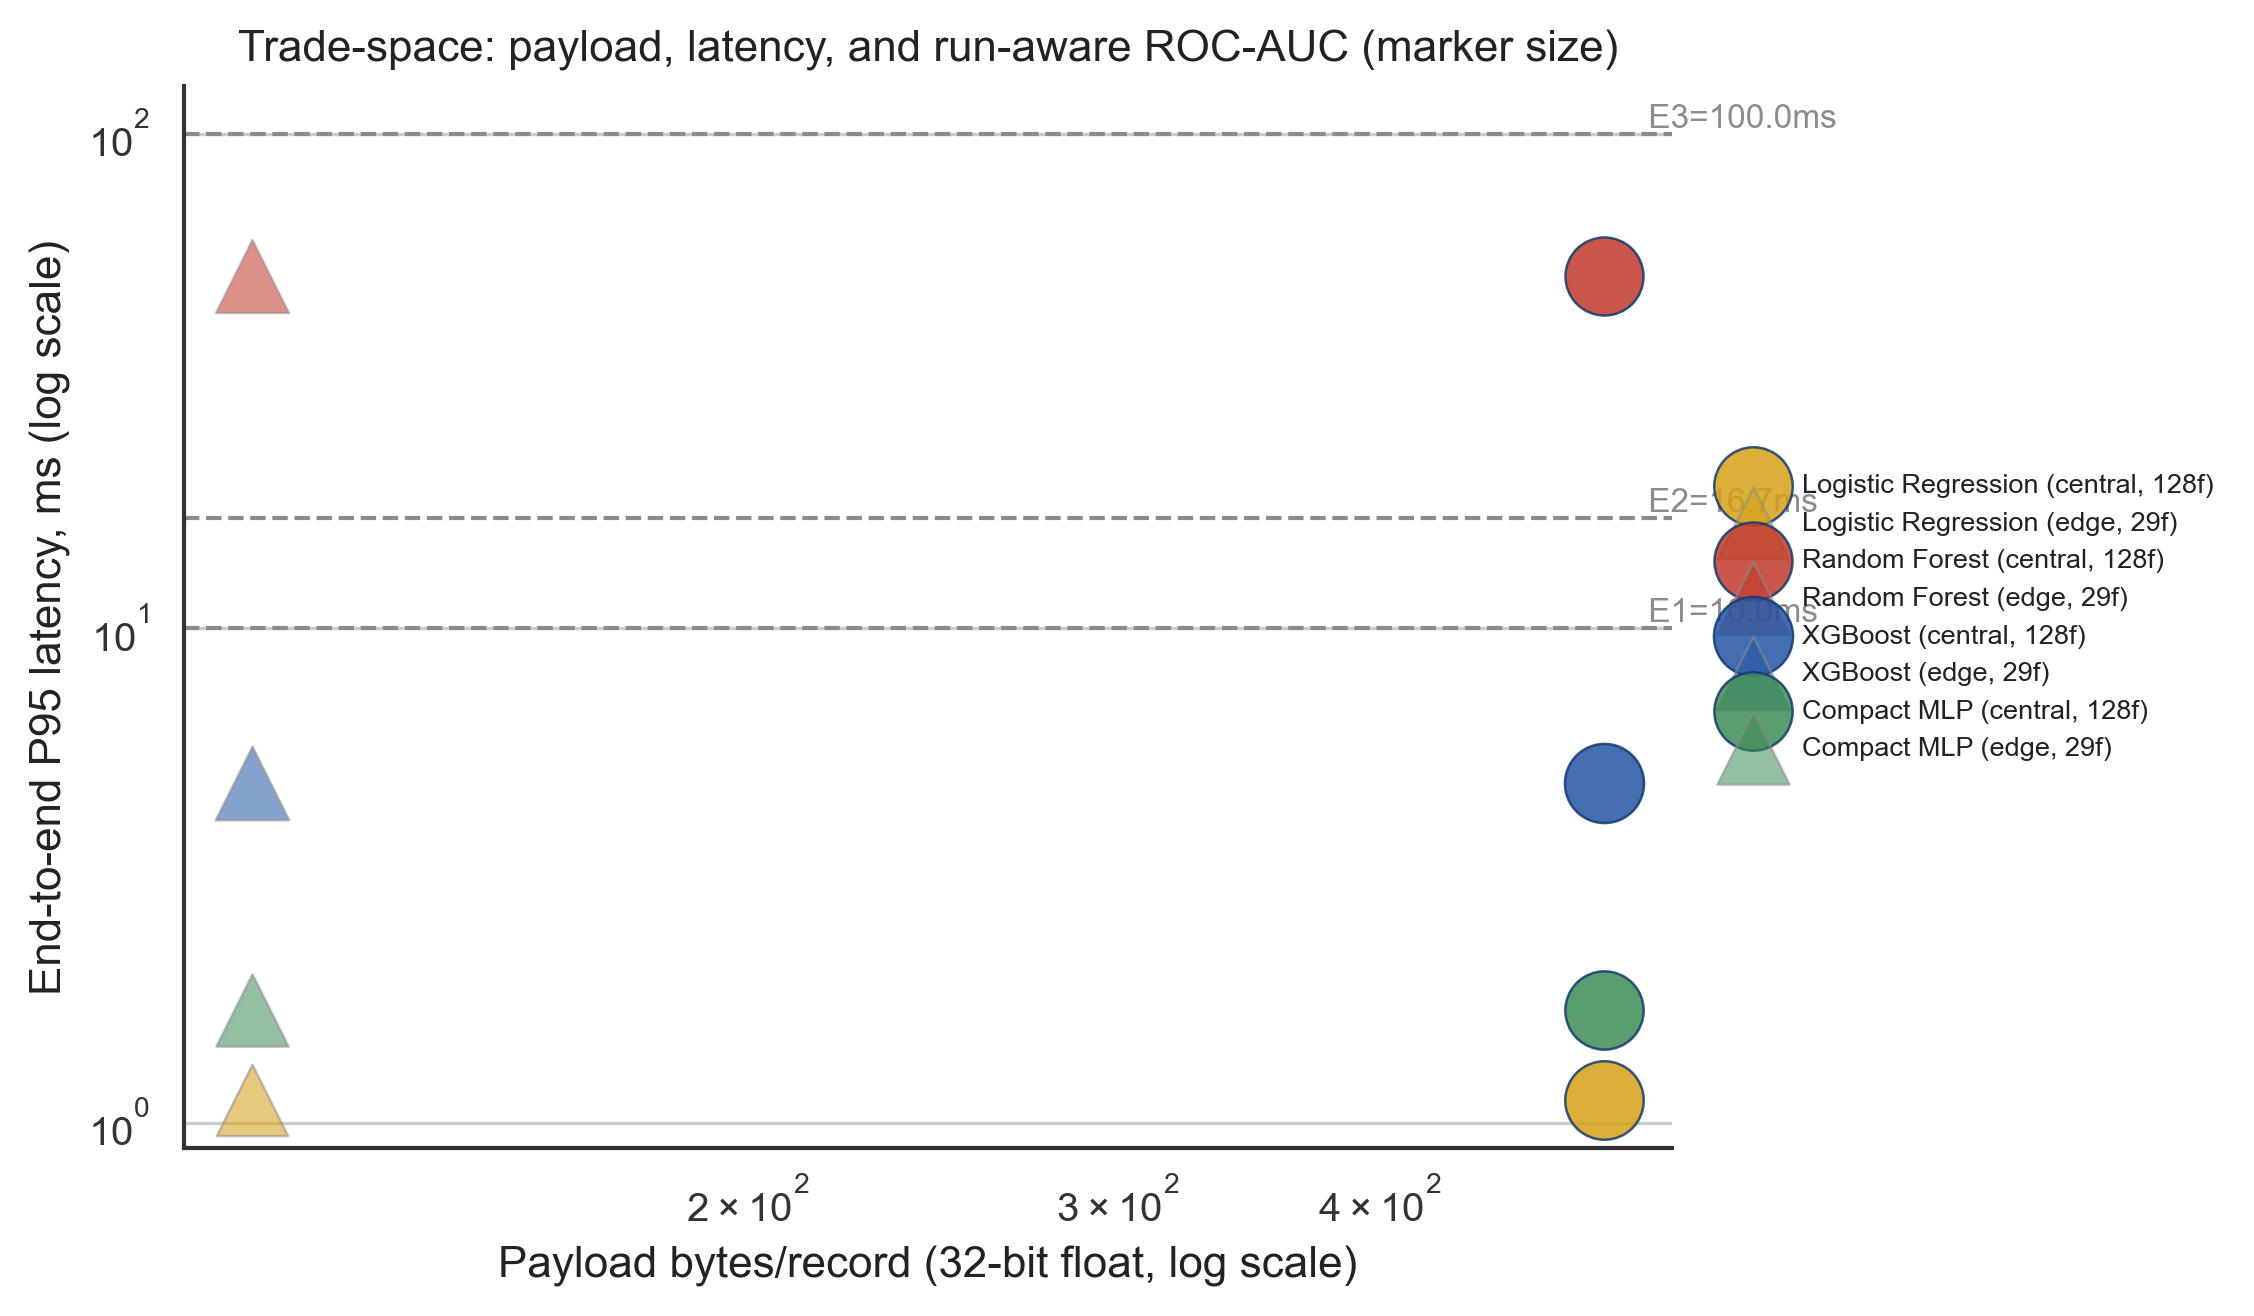
\includegraphics[width=\linewidth]{fig_tradespace.png}
\caption{Payload (bytes/record) versus P95 end-to-end latency (ms) for each model at the 128-feature (central) and edge-visible (29-feature) budgets; marker size encodes run-aware ROC-AUC; horizontal lines mark envelopes E1--E3.}
\label{fig:tradespace}
\end{figure}

\begin{table}[!t]
\caption{Run-aware quality, latency, and payload by feature budget.}
\label{tab:feature-budget}
\centering
\scriptsize
\begin{tabular}{lrrrr}
\toprule
Budget & F1 & AUC & P95 ms & Payload (B) \\
\midrule
128 & 0.813 & 0.687 & 14.8 & 512 \\
64 (ranked) & 0.812 & 0.683 & 7.9 & 256 \\
32 (ranked) & 0.811 & 0.670 & 4.7 & 128 \\
16 (ranked) & 0.821 & 0.691 & 4.5 & 64 \\
PMU only (116) & 0.813 & 0.687 & 4.8 & 464 \\
Cyber/log only (12) & 0.828 & 0.538 & 4.5 & 48 \\
\bottomrule
\end{tabular}
\end{table}
\emph{F1/AUC/P95 are the 4-model mean (Logistic Regression, Random Forest, XGBoost, compact MLP); ranked budgets use per-fold RandomForest-importance ranking on training data only.}

The top-16 ranked budget is the standout result: it matches or slightly exceeds the full 128-feature budget on both F1 (0.821 vs.\ 0.813) and AUC (0.691 vs.\ 0.687) while cutting payload $8\times$ (512 to 64 bytes) and P95 latency by roughly $3\times$ (14.8 to 4.5~ms, mean across models). The 64- and 32-feature ranked budgets do not show the same benefit and instead sit slightly below the full-feature AUC, so the relationship between budget size and unseen-run discrimination is non-monotonic here rather than a smooth accuracy--payload trade curve: a small, training-fold-selected feature set can generalize better across collection runs than either the full feature set or a mid-sized ranked subset, plausibly because the top-ranked features are also the most run-invariant ones. PMU-only (116 features, 464 bytes) matches full-feature performance almost exactly, confirming the 12 cyber/log features contribute little to discrimination; cyber/log-only (12 features, 48 bytes) collapses to near-chance AUC (0.538) despite retaining deceptively high F1 (0.828, driven by the attack-majority class prior), which is itself a caution against reading F1 alone as a budget-adequacy signal.

\subsection{Availability Robustness}

\begin{table*}[!t]
\caption{Run-aware ROC-AUC under availability degradation of held-out test data.}
\label{tab:robustness}
\centering
\small
\begin{tabular}{lcccccc}
\toprule
Model & Clean & 10\% Missing & 30\% Missing & Worst Relay Loss & Logs Unavailable & PMU Group Unavailable \\
\midrule
Logistic Regression & 0.687 & 0.581 & 0.543 & 0.499 & 0.672 & 0.531 \\
Random Forest & 0.677 & 0.680 & 0.659 & 0.580 & 0.674 & 0.506 \\
XGBoost & 0.702 & 0.672 & 0.617 & 0.612 & 0.699 & 0.509 \\
Compact MLP & 0.683 & 0.636 & 0.589 & 0.564 & 0.659 & 0.518 \\
Feature-space CNN & \multicolumn{6}{l}{Not evaluated (excluded; see Limitations)} \\
\bottomrule
\end{tabular}
\end{table*}

\begin{figure}[!t]
\centering
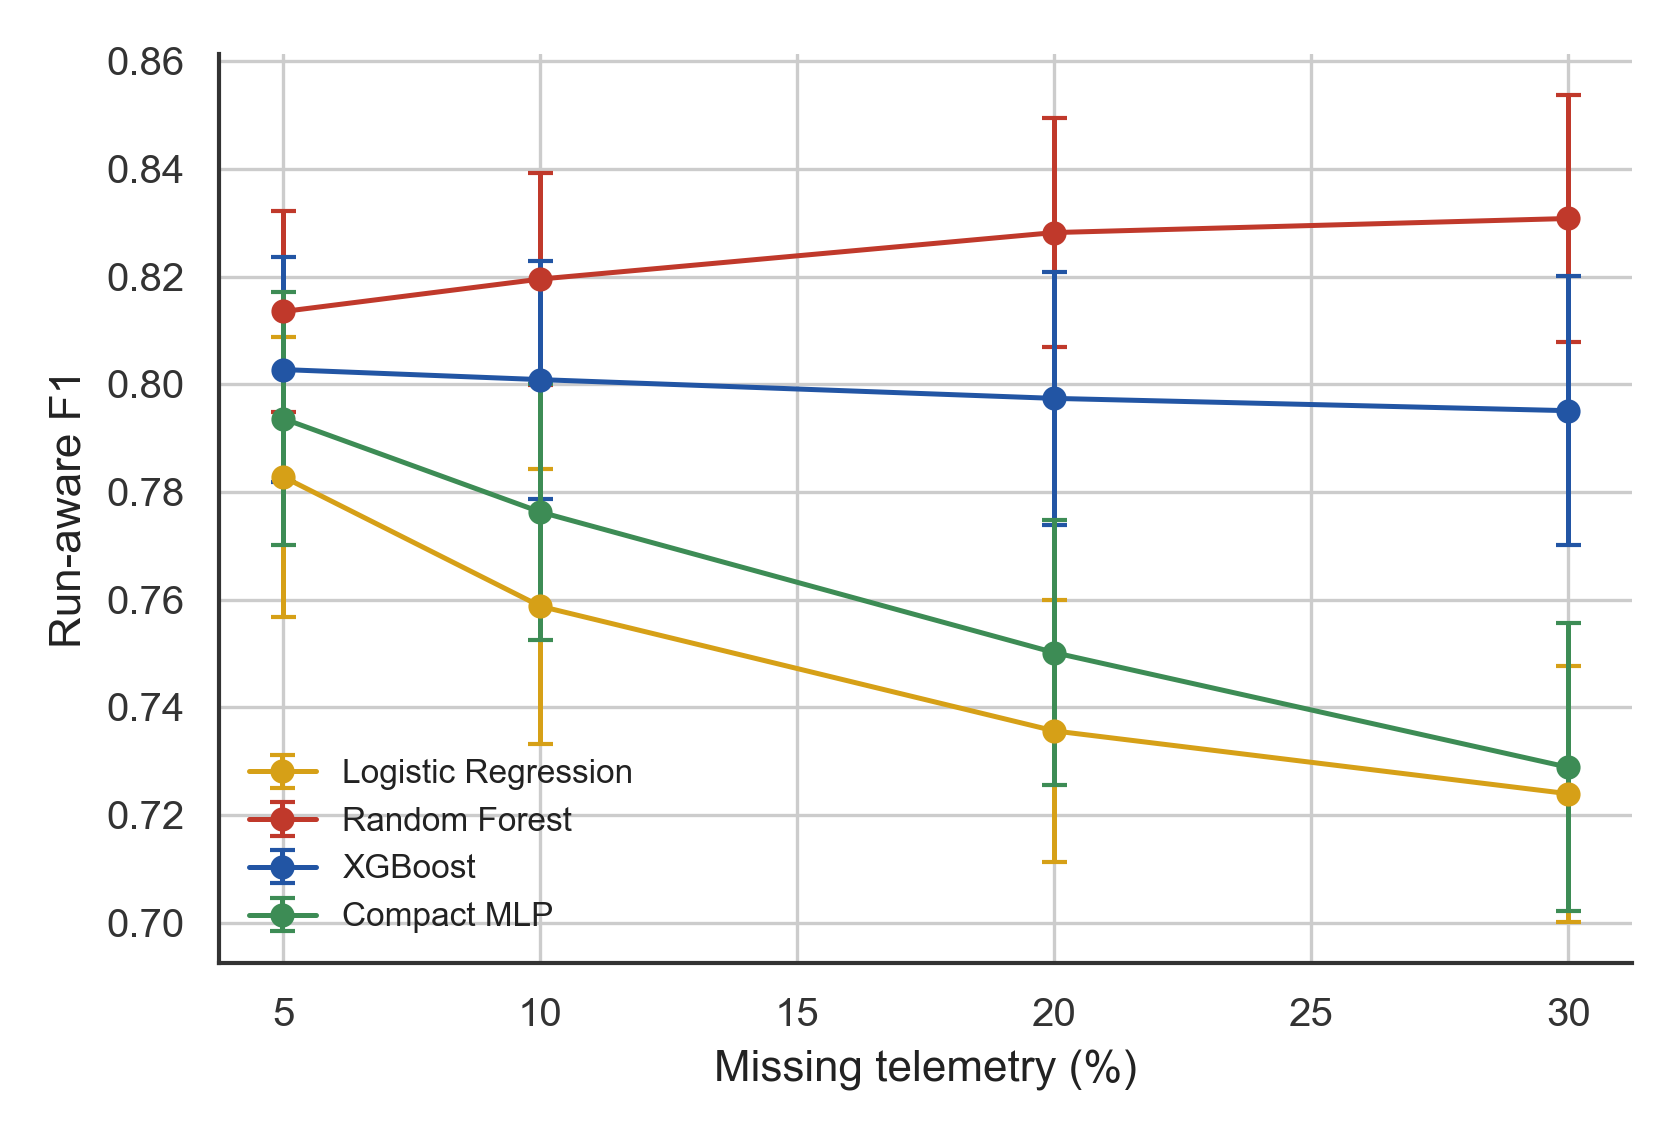
\includegraphics[width=\linewidth]{fig_missingness.png}
\caption{Run-aware F1 as missing telemetry increases from 5\% to 30\%, mean $\pm$ SD over 5 seeds and 15 folds.}
\label{fig:missingness}
\end{figure}

Complete PMU-group unavailability is by far the most damaging condition tested: masking all 116 PMU features collapses every model to near-chance discrimination (ROC-AUC 0.51--0.53), versus a comparatively mild cost from losing the 12 cyber/log features (0.66--0.70, close to clean). Among individual relays, no single relay is uniformly worst across models, but losing a model's single most-informative relay is severe for Logistic Regression (AUC falls to 0.499, i.e. to chance) and comparatively contained for XGBoost (0.612) and Random Forest (0.580). Random Forest is the most gracefully degrading model under random missingness---its F1 is nearly flat from 5\% to 30\% missing (tree splits absorb median-imputed gaps), while Logistic Regression and the compact MLP lose the most F1 over the same range.

\subsection{Edge Versus Central Placement}

\begin{table}[!t]
\caption{Placement comparison: unseen-run quality and modeled end-to-end latency.}
\label{tab:placement}
\centering
\scriptsize
\begin{tabular}{lrrr}
\toprule
Placement / condition & AUC & F1 & P95 + $d_{agg}$ ms \\
\midrule
Edge (edge-visible features) & 0.556 & 0.805 & 14.8 \\
Central, clean aggregation & 0.687 & 0.813 & 19.8 \\
Central, 10\% missing & 0.642 & 0.789 & 19.8 \\
Central, logs unavailable & 0.676 & 0.813 & 19.8 \\
Central, one relay lost (worst) & 0.564 & 0.761 & 19.8 \\
\bottomrule
\end{tabular}
\end{table}
\emph{AUC and F1 are the 4-model mean (Logistic Regression, Random Forest, XGBoost, compact MLP); latency uses the same 4-model mean P95 end-to-end compute time (dominated by Random Forest) plus $d_{agg}=5$~ms for central rows, $d_{agg}=0$ for edge.}

Averaged across models, central clean aggregation dominates edge-only visibility (AUC 0.687 vs.\ 0.556) and remains ahead of edge even under 10\% missingness or logs unavailable. The ordering flips, however, for Logistic Regression specifically: under its single worst-relay loss, central AUC falls to 0.499---at or below chance---while its edge-only AUC (0.531) is unaffected by a central aggregation failure it never depended on. So the answer to whether full central visibility always dominates is no: it dominates on average and under mild impairment, but a severe single-point aggregation failure can push a linear model below what a structurally limited edge deployment would have delivered on its own.

\subsection{Thresholds and Explanation Overhead Inside the Budget}

\begin{table}[!t]
\caption{Held-out-run alert behavior under training-selected thresholds.}
\label{tab:thresholds}
\centering
\scriptsize
\begin{tabular}{lrrr}
\toprule
Threshold rule & FPR & Recall & Alerts/1000 \\
\midrule
Fixed 0.5 & 0.755 & 0.898 & 856 \\
Max F1 & 0.724 & 0.868 & 826 \\
Max Youden $J$ & 0.410 & 0.647 & 578 \\
Constrained FPR & 0.357 & 0.592 & 524 \\
\bottomrule
\end{tabular}
\end{table}

\begin{table}[!t]
\caption{Prediction and explanation latency against envelope E3.}
\label{tab:explain}
\centering
\scriptsize
\begin{tabular}{lrrrc}
\toprule
Model & Pred. ms & SHAP ms & Total ms & Fits E3 \\
\midrule
Random Forest & 14.459 & 881.275 & 897.631 & -- \\
XGBoost & 0.125 & 1.126 & 1.263 & \checkmark \\
\bottomrule
\end{tabular}
\end{table}

Threshold selection is far from run-invariant. Random Forest's threshold is nearly rule-independent (0.617 for max-F1, max-Youden-$J$, and the 10\%-FPR constraint alike---a discrete-output artifact of averaging 200 trees), but Logistic Regression's max-F1 threshold swings from 0.0007 to 0.492 across the fifteen held-out runs (std 0.213), meaning a single fixed operating point chosen from one training set is not safely portable to another run for that model. Across models, moving from fixed 0.5 to the 10\%-constrained-FPR rule cuts alert volume from 856 to 524 per 1{,}000 records at the cost of recall (0.898 to 0.592), the expected precision--recall trade of a stricter threshold. On explanation cost: XGBoost's TreeSHAP explanation is fast enough (1.1~ms median) that prediction-plus-explanation together (1.3~ms) comfortably fits every envelope including E1, so explaining every alert is free. Random Forest's TreeSHAP is not: at 881~ms per explanation it is roughly $9\times$ over the 100~ms E3 budget and two orders of magnitude too slow for E1/E2, so explaining every record is infeasible (explaining the full 78{,}377-record test set would take on the order of 19 hours); selective strategies reduce this only in proportion to how few records are explained (e.g.\ explaining only the 25\% of records flagged high-risk still costs roughly 4.75 hours for Random Forest, versus roughly 90~seconds for XGBoost's full test set). For SHAP-based operator review, model choice---not selective-explanation strategy---is what determines whether per-alert explanation is viable at all.

\section{Discussion}

\subsection{Budgets Convert Benchmarks into Engineering Verdicts}

Reporting milliseconds and AUC in isolation invites arbitrary interpretation. Referencing standardized transfer-time classes and reporting intervals converts the same measurements into deployment verdicts: a model either sustains the inter-record interval of a synchrophasor stream or it does not. In this study the pattern is model-family, not accuracy, dependent: the linear and shallow-network models (Logistic Regression, XGBoost, compact MLP) all fit every envelope including the strict 10~ms E1 class, while Random Forest---despite being competitive on run-aware accuracy---fits only the 100~ms operational envelope E3 because batch-size-one tree-ensemble inference does not amortize. The same split reappears for explanation cost: XGBoost's TreeSHAP fits every envelope for free, Random Forest's does not fit any envelope tighter than E3 even before accounting for prediction time. A benchmark score alone would not have surfaced either fits/fails boundary.

\subsection{Run Shift and Communication Degradation Are Distinct Risks}

Run-aware evaluation measures transfer to an unseen collection; availability degradation measures resilience of the communication process. A model may survive one and fail the other, so both budgets must be reported together.

\subsection{Payload Reduction Is a Communication Decision, Not Only a Compute Decision}

Reducing the feature budget lowers payload, preprocessing work, and dependence on vulnerable channels, but aggressive reduction can remove measurements needed for unseen-run transfer. The operating point should be chosen from the full payload--latency--quality trade space rather than from accuracy alone.

\subsection{Placement Determines Which Budget Binds}

At the edge, the availability budget binds structurally; centrally, it binds stochastically through aggregation impairment while the latency budget absorbs collection delay. Central placement dominated under the conditions measured here---on average across models it retained higher accuracy than edge-only visibility even under 10\% missingness or complete log unavailability---but this dominance is conditional, not guaranteed: for Logistic Regression, losing its single most-informative relay centrally pushed accuracy to chance, below what the structurally limited edge deployment would have delivered on its own. A placement decision made only from clean-aggregation numbers would miss this failure mode entirely.

\subsection{Alert Load and Explanation Are Part of the Same Envelope}

The earlier feature-space CNN achieved high recall largely by alerting on nearly everything, which is operationally unusable regardless of latency. Alert frequency, threshold stability, and per-alert explanation cost must fit the same operational envelope as detection itself.

\section{Threats to Validity and Limitations}
\label{sec:limitations}

The study uses one benchmark from one physical testbed and does not establish transfer across utilities, vendors, or topologies; labels are binary. The files do not preserve a valid temporal sequence, so the study cannot estimate time-to-detection or early-warning capability; simulated missingness and unavailability represent feature availability at classification time, not reconstructed packet-level timing. Aggregation delays in the placement analysis are modeled assumptions, not network measurements; latency envelopes E1--E3 are citable yardsticks, not claims that the detector participates in protection signaling. Latency results depend on the reported hardware, software, and threading configuration. Payload figures exclude protocol framing. SHAP provides post-hoc attribution, not causal explanation or evidence of operator usefulness.

The feature-space 1D-CNN evaluated in prior work on this dataset is reported in Table~\ref{tab:baseline-results} for context but was excluded from every new experiment in this paper (latency, feature budgets, availability robustness, placement, thresholds, and SHAP overhead). Retraining it under this study's leave-one-run-out protocol required a CPU-only workaround for an OpenMP library conflict between PyTorch and XGBoost in our environment; under that workaround, per-fold training time made retraining it across the full robustness and placement suite impractical within the scope of this study. Its random-split and run-aware numbers in Table~\ref{tab:baseline-results} are therefore prior-work reference values, not results re-derived under the budget and placement conditions studied here, and no claim in this paper about latency, payload, or availability robustness extends to it.

\section{Conclusion}

This paper reframes SCADA intrusion detection as a real-time communications service and evaluates it against the three budgets that govern deployability: latency referenced to IEC~61850 and IEEE~C37.118 envelopes, telemetry payload determined by the transmitted feature budget, and feature availability under missing telemetry, delayed groups, and relay loss---all measured under leave-one-run-out evaluation so every number reflects an unseen collection run. Together with an edge-versus-central placement comparison and threshold and explanation overheads, the result is a fits-or-fails map intended to tell a communication engineer what the network must deliver for lightweight detection to be viable. Because the benchmark is not a continuous time series, conclusions are limited to low-latency record-level detection rather than temporal early attack detection.

\balance

\begin{thebibliography}{99}

\bibitem{sahani2023machine}
N. Sahani, R. Zhu, J.-H. Cho, and C.-C. Liu,
``Machine learning-based intrusion detection for smart grid computing: A survey,''
\emph{ACM Transactions on Cyber-Physical Systems}, vol. 7, no. 2, pp. 1--31, 2023.

\bibitem{alimi2021review}
O. A. Alimi, K. Ouahada, A. M. Abu-Mahfouz, S. Rimer, and K. O. A. Alimi,
``A review of research works on supervised learning algorithms for SCADA intrusion detection and classification,''
\emph{Sustainability}, vol. 13, no. 17, p. 9597, 2021.

\bibitem{pan2015hybrid}
S. Pan, T. Morris, and U. Adhikari,
``Developing a hybrid intrusion detection system using data mining for power systems,''
\emph{IEEE Transactions on Smart Grid}, vol. 6, no. 6, pp. 3104--3113, 2015.

\bibitem{upadhyay2021intrusion}
D. Upadhyay, J. Manero, M. Zaman, and S. Sampalli,
``Intrusion detection in SCADA based power grids: Recursive feature elimination model with majority vote ensemble algorithm,''
\emph{IEEE Transactions on Network Science and Engineering}, vol. 8, no. 3, pp. 2559--2574, 2021.

\bibitem{yang2019deep}
H. Yang, L. Cheng, and M. C. Chuah,
``Deep-learning-based network intrusion detection for SCADA systems,''
in \emph{Proc. IEEE Conf. Communications and Network Security}, 2019, pp. 1--7.

\bibitem{wang2022lightweight}
Z. Wang, Z. Li, D. He, and S. Chan,
``A lightweight approach for network intrusion detection in industrial cyber-physical systems based on knowledge distillation and deep metric learning,''
\emph{Expert Systems with Applications}, vol. 206, p. 117671, 2022.

\bibitem{shao2024automated}
J.-M. Shao, G.-Q. Zeng, K.-D. Lu, G.-G. Geng, and J. Weng,
``Automated federated learning for intrusion detection of industrial control systems based on evolutionary neural architecture search,''
\emph{Computers \& Security}, vol. 143, p. 103910, 2024.

\bibitem{chen2016xgboost}
T. Chen and C. Guestrin,
``XGBoost: A scalable tree boosting system,''
in \emph{Proc. 22nd ACM SIGKDD Int. Conf. Knowledge Discovery and Data Mining}, 2016, pp. 785--794.

\bibitem{iec61850-5}
IEC, ``Communication networks and systems for power utility automation --- Part 5: Communication requirements for functions and device models,'' IEC 61850-5, 2013.
% AUTHORS: verify edition/year and the transfer-time class values you cite in Sec. IV-A against the actual standard text.

\bibitem{iec61850-90-4}
IEC, ``Communication networks and systems for power utility automation --- Part 90-4: Network engineering guidelines,'' IEC TR 61850-90-4, 2020.
% AUTHORS: verify edition/year.

\bibitem{ieee-c37118}
IEEE, ``IEEE standard for synchrophasor data transfer for power systems,'' IEEE Std C37.118.2-2011, 2011.
% AUTHORS: verify part (measurement .1 vs data transfer .2) and reporting-rate statement.

\bibitem{substation-comms-survey}
\resulttodo{AUTHORS: add one survey on digital-substation communication engineering / latency verification (e.g., a 61850 process-bus performance study).}

\bibitem{edge-ids-survey}
\resulttodo{AUTHORS: add one edge/lightweight IDS survey or representative paper.}

\bibitem{tinyml-ids}
\resulttodo{AUTHORS: add one TinyML / resource-constrained detection reference.}

\bibitem{missing-features-ml}
\resulttodo{AUTHORS: add one reference on inference-time missing features / feature robustness in tabular ML.}

\bibitem{arp2022dodo}
D. Arp, E. Quiring, F. Pendlebury, A. Warnecke, F. Pierazzi, C. Wressnegger, L. Cavallaro, and K. Rieck,
``Dos and don'ts of machine learning in computer security,''
in \emph{Proc. 31st USENIX Security Symposium}, 2022, pp. 3971--3988.
% AUTHORS: verify page range.

\bibitem{kadri2025physics}
B. Kadri, L. Sliman, A. Alsaedi, J. Abdella, and Z. Farah,
``Physics-aware hybrid estimator for dynamic power system dataset generation and cyber attack simulation,''
\emph{IEEE Access}, 2025.

\bibitem{cibin2026dataset}
N. Cibin, N. Kabbara, A. Presekal, I. Semertzis, V. Rajkumar, H. Goyel, P. Palensky, and A. \c{S}tefanov,
``Cyber-physical power system dataset for cyber security of digital substations,''
\emph{IEEE Access}, 2026.

\bibitem{huang2023beyond}
F. Huang, W. Shangguan, Q. Li, L. Li, and Y. Zhang,
``Beyond prediction: An integrated post-hoc approach to interpret complex models in hydrometeorology,''
\emph{Environmental Modelling \& Software}, vol. 167, p. 105762, 2023.

\end{thebibliography}

\end{document}
